\subsubsection*{Project 3: Modeling oxygen insertion in one-dimensional channels of shafarzikite-like structures}\label{deLaune}
 Recent study of schafarzikite-like ($\textrm{FeSb}_2\textrm{O}_4$) materials have been shown to store relatively large amounts of oxygen (~3.5\% mass)
within the structure at low temperatures (~350 $^{\circ}$C) without decomposition, leading to new possibilities as potential oxygen storage materials \cite{Laune2017}.


\begin{figure}[h]
  \label{fesb2o4}
  \begin{tabular}{ccc}
    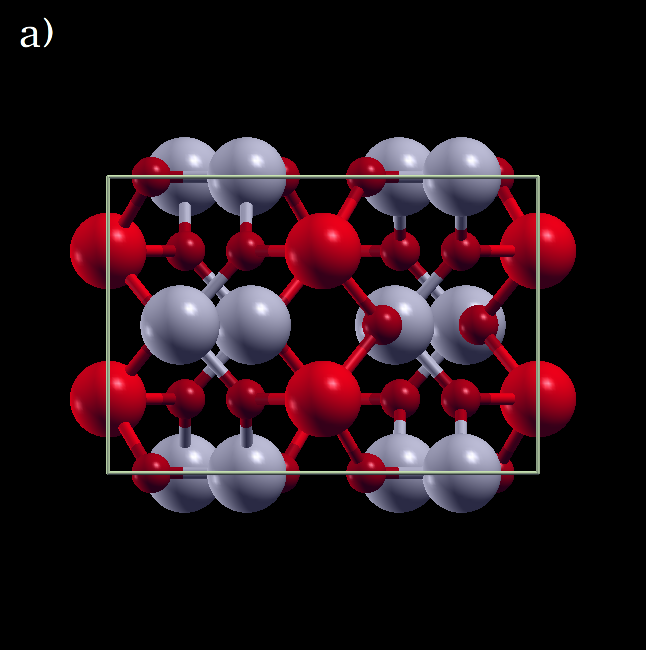
\includegraphics[width=0.33\textwidth]{graphics/fesb2o4_xaxis.png} &
    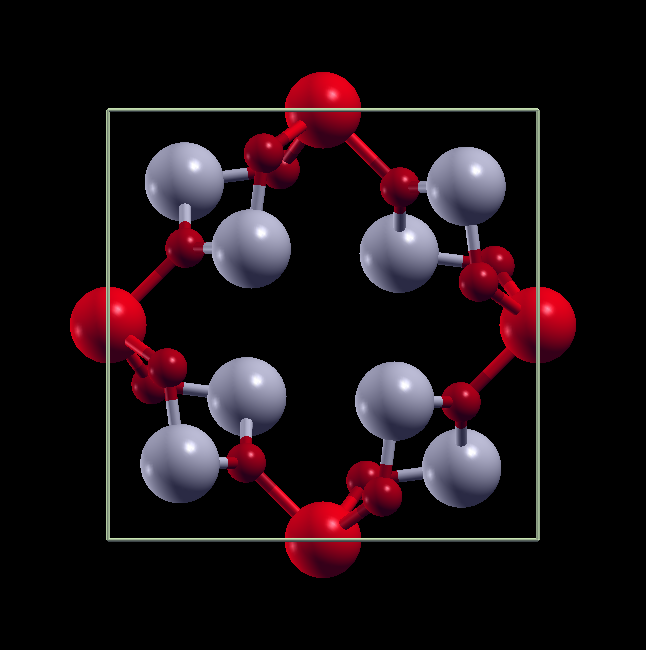
\includegraphics[width=0.33\textwidth]{graphics/fesb2o4_zaxis.png} &
    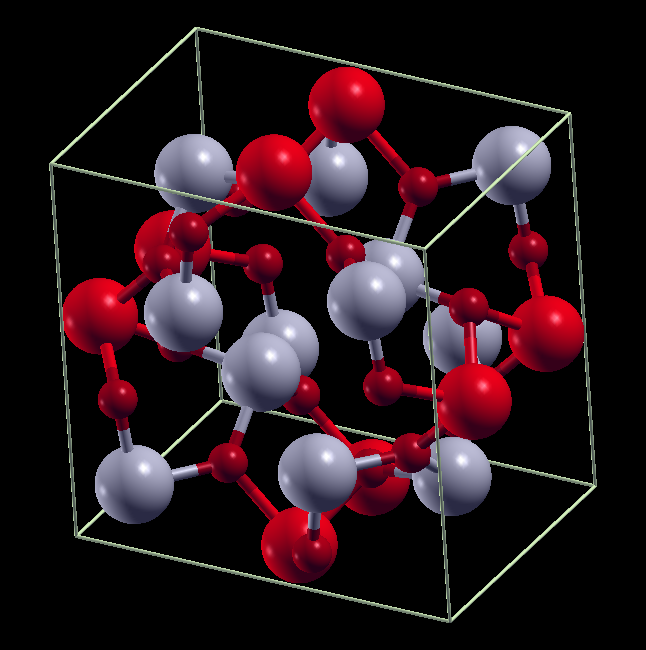
\includegraphics[width=0.33\textwidth]{graphics/fesb2o4_tilted.png} \\
  \end{tabular}
  \caption{\textbf{Schafarzikite} Fe atoms: \color{red} red \color{black} O atoms: \color{BrickRed} dark red \color{black} Sb atoms: \color{Gray} gray \color{black}. Showing the orientations for (a) (100) (b) (001) and (c) (111).  }

 
\end{figure}


In Figure \ref{fesb2o4}, we show the shafarzikite structure along different axes. The Fe atoms are show as \color{red} red \color{black}, the O atoms are show as \color{BrickRed} dark red \color{black} and the Sb atoms are shown as \color{Gray} gray \color{black}. Oxygen insertion into cobalt and lead doped derivatives of
shafarzikite show promise in applications of electro-catalysis due to their unique
1-D cation channels with high peroxide anion mobility and potential for high,
directed electronic conductivity \cite{Laune2017}. For this project, we plan to analyze the neutron
scattering data first with RMC modeling to clarify the structures that occur 
before and after oxidization and also variants of the material with different
doping agents.


Structures generated from the RMC modeling can then be used to construct nudged
elastic band \cite{Henkelman2000, Henkelman2000a} calculations using density functional theory to determine the minimum energy pathway during the oxidation process. This would allow one to know the energetic barrier at the transition state.  Results from this study would
help in clarifying the proposed defect cluster produced by the low temperature
oxidation reaction and help in proposing new chemistry of schafarzikite-like materials to optimize oxygen storage. 





 


